\documentclass[12pt]{exam}
\usepackage[colorlinks]{hyperref}
\usepackage{enumitem}
\usepackage{float}
\usepackage{graphicx}
\usepackage{listings}
\usepackage{multicol}
\usepackage{xcolor}

\graphicspath{ {./images/} }

\lstset{
    showstringspaces=false,
    breaklines=true,
    basicstyle=\footnotesize,
    commentstyle=\color{gray}
}

\begin{document}
\noindent
Derrick Lee\\
Lab 3\\
CSCI 180\\
\today\\

\section{}

Running shellcodetest results in a shell being run by a buffer overflow.  The
shell is run by a buffer overflow attack, modifying the return address to
execute given code to run a shell.

\section{}

Modified variables:

\begin{lstlisting}[language=python]
    D = 36
    content[D+0] = 0xB8
    content[D+1] = 0xF0
    content[D+2] = 0xFF
    content[D+3] = 0xBF
\end{lstlisting}

The found value of D was 36.  This is calculated by finding the difference
between the address of EBP (\lstinline{0xbffff0a8}) and buffer
(\lstinline{0xbffff088}), then adding 4. 

$$\mathtt{0xbffff0a8} - \mathtt{0xbffff088} = \mathtt{0x20} \equiv 32$$
$$32 + 4 = 36$$

To find the address, the EBP address
was used in the debugger and just offset slightly to be a higher number
(\lstinline{0xbffff0a8} to \lstinline{0xbffff0b8})

\vspace*{.2in}
\noindent
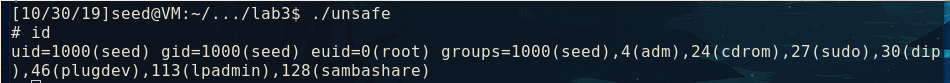
\includegraphics[width=\textwidth]{q2}

\section{}

Despite \lstinline{/bin/dash} having countermeasures for setuid attacks, adding
the given code to set the euid to 0 before running the \lstinline{/bin/dash}
shell results in a root shell.  The countermeasure is to set the euid same as
the real uid, and when adding the code to set the uid as 0, setting the euid the
same would result still having root access.

\vspace*{.2in}
\noindent
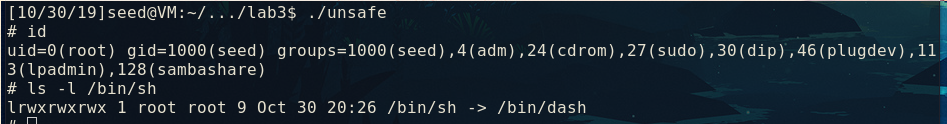
\includegraphics[width=\textwidth]{q3}

\section{}

Running the previous attack resulted in a Segmentation fault.  This is because
with a randomized virtualized address space, it is more difficult to figure out
what address to use for the malicious return address.

\section{}

After running the script to brute force the buffer overflow attack resulted in
a root shell.  Since the virtual address space is randomized, running the
program repeatedly will eventually result in the malicious return address to be
correct and execute the malicious shellcode.

\vspace*{.2in}
\noindent
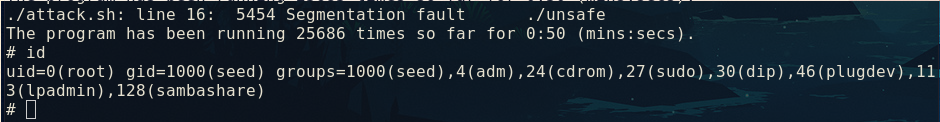
\includegraphics[width=\textwidth]{q5}

\end{document}
